\chapter{Path Loss: From Friis to 3GPP Urban Macro}
\label{ch:pathloss}

\begin{defbox}[In this chapter you will learn]
\begin{itemize}
 \item how the Friis transmission equation follows from two simple ideas---power density and effective aperture;
 \item why real environments need path-loss models beyond free space, and what the \emph{breakpoint distance} means;
 \item the 3GPP TR~38.901 Urban Macro (UMa) line-of-sight and non-line-of-sight formulas that Amber implements, with all constants explained;
 \item how Amber applies medium attenuation, and two subtle behaviours of the code near the base station.
\end{itemize}
\end{defbox}

\section{Free-space propagation: Friis}
\label{sec:friis}

Two ideas, both geometric, give the free-space law.

\paragraph{Idea 1: power density.}
An isotropic transmitter of power $P_t$ spreads its power over a sphere of
area $4\pi d^2$ at distance $d$. With antenna gain $G_t$ toward the receiver the power
density is
\[
 S \;=\; \frac{P_t\,G_t}{4\pi d^2}\qquad[\mathrm{W/m^2}].
\]

\paragraph{Idea 2: effective aperture.}
A receiving antenna of gain $G_r$ intercepts power from a passing wave as if it
had an \emph{effective area}
\[
 A_e \;=\; \frac{G_r\lambda^2}{4\pi},\qquad \lambda=\frac{c}{f_c}.
\]
This shows an interesting fact: at a given gain, a lower frequency means a larger
effective area, so a $\SI{924}{MHz}$ antenna ($\lambda=\SI{0.325}{m}$) captures
$\approx$10 times more power than a $\SI{3}{GHz}$ one of the same gain. Multiply the two:
\begin{equation}
 P_r \;=\; S\,A_e \;=\; P_t\,G_t\,G_r\left(\frac{\lambda}{4\pi d}\right)^{\!2}.
\label{eq:friis}
\end{equation}
This is the \emph{Friis transmission equation} \citep{friis1946}. The last factor,
\begin{equation}
 L_{\mathrm{FS}}(d)=\left(\frac{\lambda}{4\pi d}\right)^{2},\qquad
 \mathrm{PL}_{\mathrm{FS}}(d)=20\log_{10}\frac{4\pi d}{\lambda}\ \mathrm{dB},
\label{eq:fspl}
\end{equation}
is the \emph{free-space path loss}. It is exactly Amber's \code{fspl_lin}. In
convenient units, $\mathrm{PL}_{\mathrm{FS}}=32.45+20\log_{10}f_{\mathrm{MHz}}+20\log_{10}d_{\mathrm{km}}$.
At $\SI{924}{MHz}$ the loss at $\SI{1}{m}$ is $\SI{31.76}{dB}$, and every doubling of
distance costs $20\log_{10}2=\SI{6.02}{dB}$ more.

\begin{keyidea}[A common misconception]
Free-space ``loss'' is not absorption. No energy disappears; it simply
\emph{spreads out}. The $\lambda^2$ in the formula comes from the receive
aperture, not from the medium: path loss at a fixed distance grows with
frequency because the receiving antenna gets \emph{smaller}.
\end{keyidea}

\begin{example}[Free space at $\SI{20}{m}$]
$\lambda=3\times10^{8}/924\times10^{6}=\SI{0.3247}{m}$.
$\mathrm{PL}_{\mathrm{FS}}(20)=20\log_{10}(4\pi\cdot20/0.3247)=20\log_{10}(774)=\SI{57.78}{dB}$.
\end{example}

\section{Beyond free space}
\label{sec:beyondfs}

Free space is the best case. In a real street the wave also reflects from the ground and
buildings, is blocked by obstacles, and diffracts around edges. Empirically one
finds that received power falls as $d^{-n}$ with a \emph{path-loss exponent} $n$
ranging from about 2 (open) to 4--6 (cluttered). The simplest physical
mechanism that makes $n=4$ is the \emph{two-ray ground reflection}: the direct
ray and its reflection from the ground interfere destructively beyond a
\emph{breakpoint distance} $d_{BP}\approx4h_th_r/\lambda$ (for antenna heights $h_t,h_r$); inside it the
loss is nearly free-space ($n\approx2$) and outside it is steeper ($n\approx4$).
This ``two-slope'' behaviour is built into the 3GPP urban macro model.

\section{3GPP TR 38.901 Urban Macro (UMa)}
\label{sec:uma}

3GPP's channel-model report TR~38.901 \citep{3gpp38901} specifies a statistical
path-loss formula for every deployment scenario for carrier frequencies between
$0.5$ and $\SI{100}{GHz}$. Amber implements the \textbf{UMa} scenario in
\codew{urban_macro_loss_db_38_901}. Let $f_c$ be in GHz, $h_{BS}$ the
base-station height (default $\SI{25}{m}$) and $h_{UT}$ the node height
(default $\SI{1.5}{m}$). The code defines
\begin{align}
 d_{3D}&=\sqrt{d_{2D}^2+(h_{BS}-h_{UT})^2}\quad(\text{clamped to}\ge\SI{10}{m}),\\
 d'_{BP}&=\frac{4\,(h_{BS}-1)\,(h_{UT}-1)\,f_c}{c}\quad[f_c\ \text{in Hz in the code}],
\end{align}
where the ``$-1$'' is the effective environment height $h_E=\SI{1}{m}$. For
the demo's heights $d'_{BP}=4\cdot24\cdot0.5\cdot924\times10^{6}/3\times10^{8}=\SI{147.8}{m}$.

\paragraph{Line of sight (LOS).} The loss has two slopes:
\begin{align}
 \mathrm{PL}_1 &= 28.0+22\log_{10}d_{3D}+20\log_{10}f_c, && 10\,\mathrm{m}\le d_{2D}\le d'_{BP},\label{eq:pl1}\\
 \mathrm{PL}_2 &= 28.0+40\log_{10}d_{3D}+20\log_{10}f_c-9\log_{10}\!\big(d_{BP}'^{\,2}+(h_{BS}-h_{UT})^2\big), && d_{2D}> d'_{BP}.\label{eq:pl2}
\end{align}
Inside the breakpoint the exponent is $2.2$ (close to free space); outside it is
$4.0$. The last term of $\mathrm{PL}_2$ makes the curve continuous at $d'_{BP}$.

\paragraph{Non line of sight (NLOS).} The 3GPP formula is
\begin{equation}
 \mathrm{PL}'_{\mathrm{NLOS}}=13.54+39.08\log_{10}d_{3D}+20\log_{10}f_c-0.6\,(h_{UT}-1.5),
\end{equation}
and the model uses $\mathrm{PL}_{\mathrm{NLOS}}=\max\!\big(\mathrm{PL}_{\mathrm{LOS}},\,\mathrm{PL}'_{\mathrm{NLOS}}\big)$ so that NLOS is never better than LOS. The
code selects LOS or NLOS with the single flag \codew{CoverageMap.los}; there is no
probabilistic LOS/NLOS switching with distance.

\begin{figure}[t]
\centering
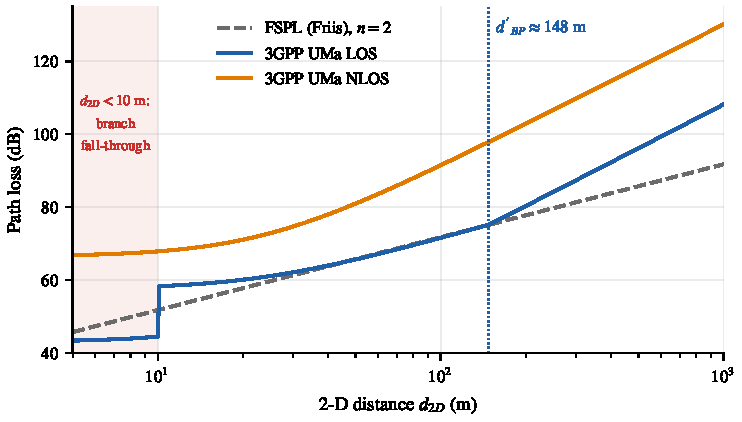
\includegraphics[width=0.85\linewidth]{fig_pathloss}
\caption{Path loss at $\SI{924}{MHz}$ with $h_{BS}=\SI{25}{m}$, $h_{UT}=\SI{1.5}{m}$, computed by Amber's own functions. Free space (dashed) and UMa LOS agree closely up to the breakpoint $d'_{BP}\approx\SI{148}{m}$, after which LOS steepens to a $40$~dB/decade slope. NLOS is $\approx11$--$22$~dB worse. The shaded region at left marks the code's non-physical behaviour below $\SI{10}{m}$ (see the reality check below).}
\label{fig:pathloss}
\end{figure}

\begin{center}
\small
\renewcommand{\arraystretch}{1.08}
\begin{tabular}{@{}rrrrr@{}}
\toprule
$d_{2D}$ (m) & $d_{3D}$ (m) & FSPL$(d_{2D})$ (dB) & UMa LOS (dB) & UMa NLOS (dB)\\
\midrule
 20 & 30.9 & 57.8 & 60.1 & 71.1\\
 30 & 38.1 & 61.3 & 62.1 & 74.6\\
 50 & 55.2 & 65.7 & 65.6 & 80.9\\
100 & 102.7 & 71.8 & 71.6 & 91.5\\
148 & 149.7 & 75.2 & 75.2 & 97.9\\
300 & 300.9 & 81.3 & 87.3 & 109.7\\
500 & 500.6 & 85.7 & 96.1 & 118.4\\
1000 & 1000.3 & 91.8 & 108.2 & 130.1\\
\bottomrule
\end{tabular}
\end{center}
\noindent\emph{Generated by calling Amber's \code{fspl_lin} and \codew{urban_macro_loss_db_38_901}.}

\begin{example}[Path loss at $\SI{100}{m}$ by hand]
$d_{3D}=\sqrt{100^2+23.5^2}=\SI{102.72}{m}$, below the breakpoint, so Eq.~\eqref{eq:pl1}:
$28+22\log_{10}102.72+20\log_{10}0.924=28+44.26-0.69=\SI{71.57}{dB}$, matching the
table and the downlink budget of the demo's Node~2 (Chapter~\ref{ch:decibels}).
\end{example}

\section{Medium attenuation}

\codew{compute_rx_power_watts} accepts an optional \codew{extra_np_per_m}, a
medium attenuation $\alpha$ in nepers per metre, and multiplies the received
power by $\e^{-\alpha d}$. Two remarks. First, in electromagnetics a ``neper
per metre'' usually quantifies attenuation of the field \emph{amplitude}
($\SI{8.686}{dB/m}$ per Np/m); because Amber applies the factor to
\emph{power}, its $\alpha$ corresponds to $4.343\,\alpha$~dB/m. Second, the
attenuation is applied once per hop, so a backscatter link suffers it \emph{twice}.
It is zero by default.

\section{What Amber assumes about the channel}

Everything in this chapter is a \emph{deterministic, static} function of
distance and angles. There is no small-scale fading (Rayleigh/Rician), no
log-normal shadow fading (3GPP specifies $\sigma_{SF}$ of several dB for UMa),
no multipath delay spread, no frequency selectivity and no
mobility. This is a conscious system-level simplification: it makes link budgets
computable \emph{once} (Chapter~\ref{ch:des}) and results repeatable, at the
price of not reproducing the variability of real channels.

\begin{reality}[Two behaviours of the path-loss code near the mast]
\textbf{(1) A $\SI{14}{dB}$ step at $\SI{10}{m}$.} The LOS formula selects
$\mathrm{PL}_1$ only for $10\le d_{2D}\le d'_{BP}$ (the range in which 3GPP defines
it). For $d_{2D}<\SI{10}{m}$ the code falls through to the \emph{post-breakpoint}
branch $\mathrm{PL}_2$. The result at $\SI{5}{m}$ is $\SI{43.4}{dB}$, whereas
$\mathrm{PL}_1$ would give $\SI{57.7}{dB}$; the curve jumps by $\SI{13.8}{dB}$ between
$\SI{9.99}{m}$ and $\SI{10}{m}$ (Figure~\ref{fig:pathloss}). We measured this directly.
Keep nodes at least $\SI{10}{m}$ (horizontally) from a mast. Note that the shipped custom-protocol demo
places nodes from $\SI{5}{m}$ outward, so a few of its nodes enjoy this extra $\sim\SI{14}{dB}$.

\textbf{(2) Free space uses the horizontal distance.} In
\codew{pathloss="fspl"} mode the function receives $d_{2D}$, not the slant range
$d_{3D}$: the $\SI{25}{m}$ mast height is ignored. At $d_{2D}=\SI{5}{m}$ this understates
the loss by $14$~dB; at $\SI{100}{m}$ by only $\SI{0.2}{dB}$. The UMa model does
use $d_{3D}$ internally.
\end{reality}

\begin{codemap}
\small
\begin{tabularx}{\linewidth}{@{}>{\ttfamily}p{5.2cm}X@{}}
\toprule
\normalfont\bfseries Concept & \normalfont\bfseries Code (\file{amber/propagation.py})\\
\midrule
Friis, Eq.~\eqref{eq:friis}, \eqref{eq:fspl} & \code{fspl_lin}, \codew{compute_rx_power_watts}\\
UMa LOS/NLOS & \codew{urban_macro_loss_db_38_901}\\
Model selection & \code{pathloss} string: \code{"fspl"} or \code{"macro"}/\code{"3gpp"}/\code{"urban"}\\
Medium attenuation & factor \codew{np.exp(-extra_np_per_m * distance_m)}\\
\bottomrule
\end{tabularx}
\end{codemap}

\section{Chapter summary}
\begin{itemize}
 \item Friis: $P_r=P_tG_tG_r(\lambda/4\pi d)^2$---spreading plus a $\lambda^2$ aperture; $\mathrm{PL}_{FS}(\SI{1}{m},\SI{924}{MHz})=\SI{31.76}{dB}$.
 \item UMa LOS has exponent $2.2$ before and $4.0$ after the breakpoint $d'_{BP}=4(h_{BS}-1)(h_{UT}-1)f_c/c$; NLOS is $\max(\text{LOS},\ \text{NLOS}')$.
 \item Amber's channel is deterministic and static: no fading or shadowing.
 \item Beware $d_{2D}<\SI{10}{m}$ (a $14$~dB discontinuity) and the horizontal-distance convention in FSPL mode.
\end{itemize}

\section*{Exercises}
\begin{exercise}
Derive Eq.~\eqref{eq:friis} from the two ideas of Section~\ref{sec:friis}, and then compute the free-space loss at $\SI{924}{MHz}$ and $\SI{3.5}{GHz}$ for $\SI{50}{m}$ with $G_r=G_t=1$. Why is the second larger?
\end{exercise}
\begin{exercise}
Compute $d'_{BP}$ for $h_{BS}=\SI{30}{m}$, $h_{UT}=\SI{2}{m}$ at $\SI{2}{GHz}$. Is a node at $d_{2D}=\SI{200}{m}$ before or after the breakpoint?
\end{exercise}
\begin{exercise}
Using Eq.~\eqref{eq:pl2}, compute the UMa LOS loss at $d_{2D}=\SI{300}{m}$ for the demo parameters ($\SI{924}{MHz}$, $25$/$\SI{1.5}{m}$). Compare with the table.
\end{exercise}
\begin{exercise}
A medium attenuation of $\alpha=0.01$~Np/m is configured. What is the extra loss in dB per hop at $\SI{100}{m}$ as Amber applies it? And over the round trip of a backscatter link?
\end{exercise}
\begin{exercise}
By what factor (in dB) does the \emph{uplink} power at the base station change when a node moves from $\SI{50}{m}$ to $\SI{100}{m}$ in the LOS regime below the breakpoint, compared with the change of the \emph{downlink} power at the node?
\end{exercise}
